\documentclass[tikz]{standalone}
\usepackage{tikz}
\usepackage{amssymb}
\usetikzlibrary{positioning}
\usetikzlibrary{calc}
\usetikzlibrary{arrows,shapes,snakes,automata,petri}
\begin{document}
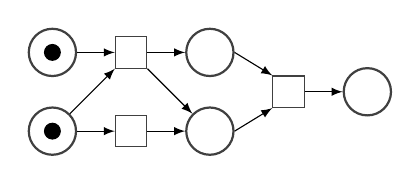
\begin{tikzpicture}
\tikzstyle{place} =[circle,thick,draw=black!75,minimum size=6mm]
\tikzstyle{transition} =[rectangle,draw=black!75,minimum size=4mm]
\tikzstyle{marking} =[circle,filled,draw=black!75,minimum size=3mm]
\node[place](init1) at (0, 0) {};
\node[place](init2) at (0,-1){};
\node[place](top) at (2,0){};
\node[place](bot) at (2,-1){};
\node[place](end) at (4,-0.5){};

\filldraw (0,0) circle (1mm);
\filldraw (0,-1) circle (1mm);

\node[transition](postinit) at (1,0){};
\draw[draw,-latex] (init1.east)--(postinit.west);
\draw[draw,-latex] (init2.north east)--(postinit.south west);
\draw[draw,-latex] (postinit.east)--(top.west);
\draw[draw,-latex] (postinit.south east)--(bot.north west);

\node[transition](postinit2) at (1,-1){};
\draw[draw,-latex] (init2.east)--(postinit2.west);
\draw[draw,-latex] (postinit2.east)--(bot.west);

\node[transition](final) at (3,-0.5){};
\draw[draw,-latex] (top.east)--(final.north west);
\draw[draw,-latex] (bot.east)--(final.south west);
\draw[draw,-latex] (final.east)--(end.west);
\end{tikzpicture}
\end{document}